%!TEX root = ../../Main.tex
\graphicspath{{Chapters/CSS_test/}}
%-------------------------------------------------------------------------------

\section{Resultater}
Projektet er resulteret i en fungerende prototype. De vigtigste funktionaliteter er blevet implementeret, heriblandt:

\begin{itemize}
	\item Aflæse tre forskellige farver(Rød, grøn og blå).
	
	\item Implementeret GUI på farveskærm
	
	\item I2C kommunikation mellem to arduinoer
	
\end{itemize}

Der er visse funktionaliteter der ikke er blevet implementeret, disse er:

\begin{itemize}
	\item Gemme data på SD kort
	
	\item Mekanik til sortering af emner

\end{itemize}

SD kort funktionalitet var godt på vej til at blive implementeret, men da det blev klart at sensor og skærm ikke ville kunne være på samme arduino, blev det nedprioriteret. Mekanikken havde ikke høj prioritet fra start, da det blev gjort klart at det ikke havde høj samhørighed med læringsmålene, dog ville det have resulteret i et mere gennemført prjoekt.
\\
På trods af visse mangler virker prototypen efter hensigten og gruppen er tilfreds med CSS.

\subsection{Visuel test af samlet sysyem}

\begin{figure}[H]
	\centering
	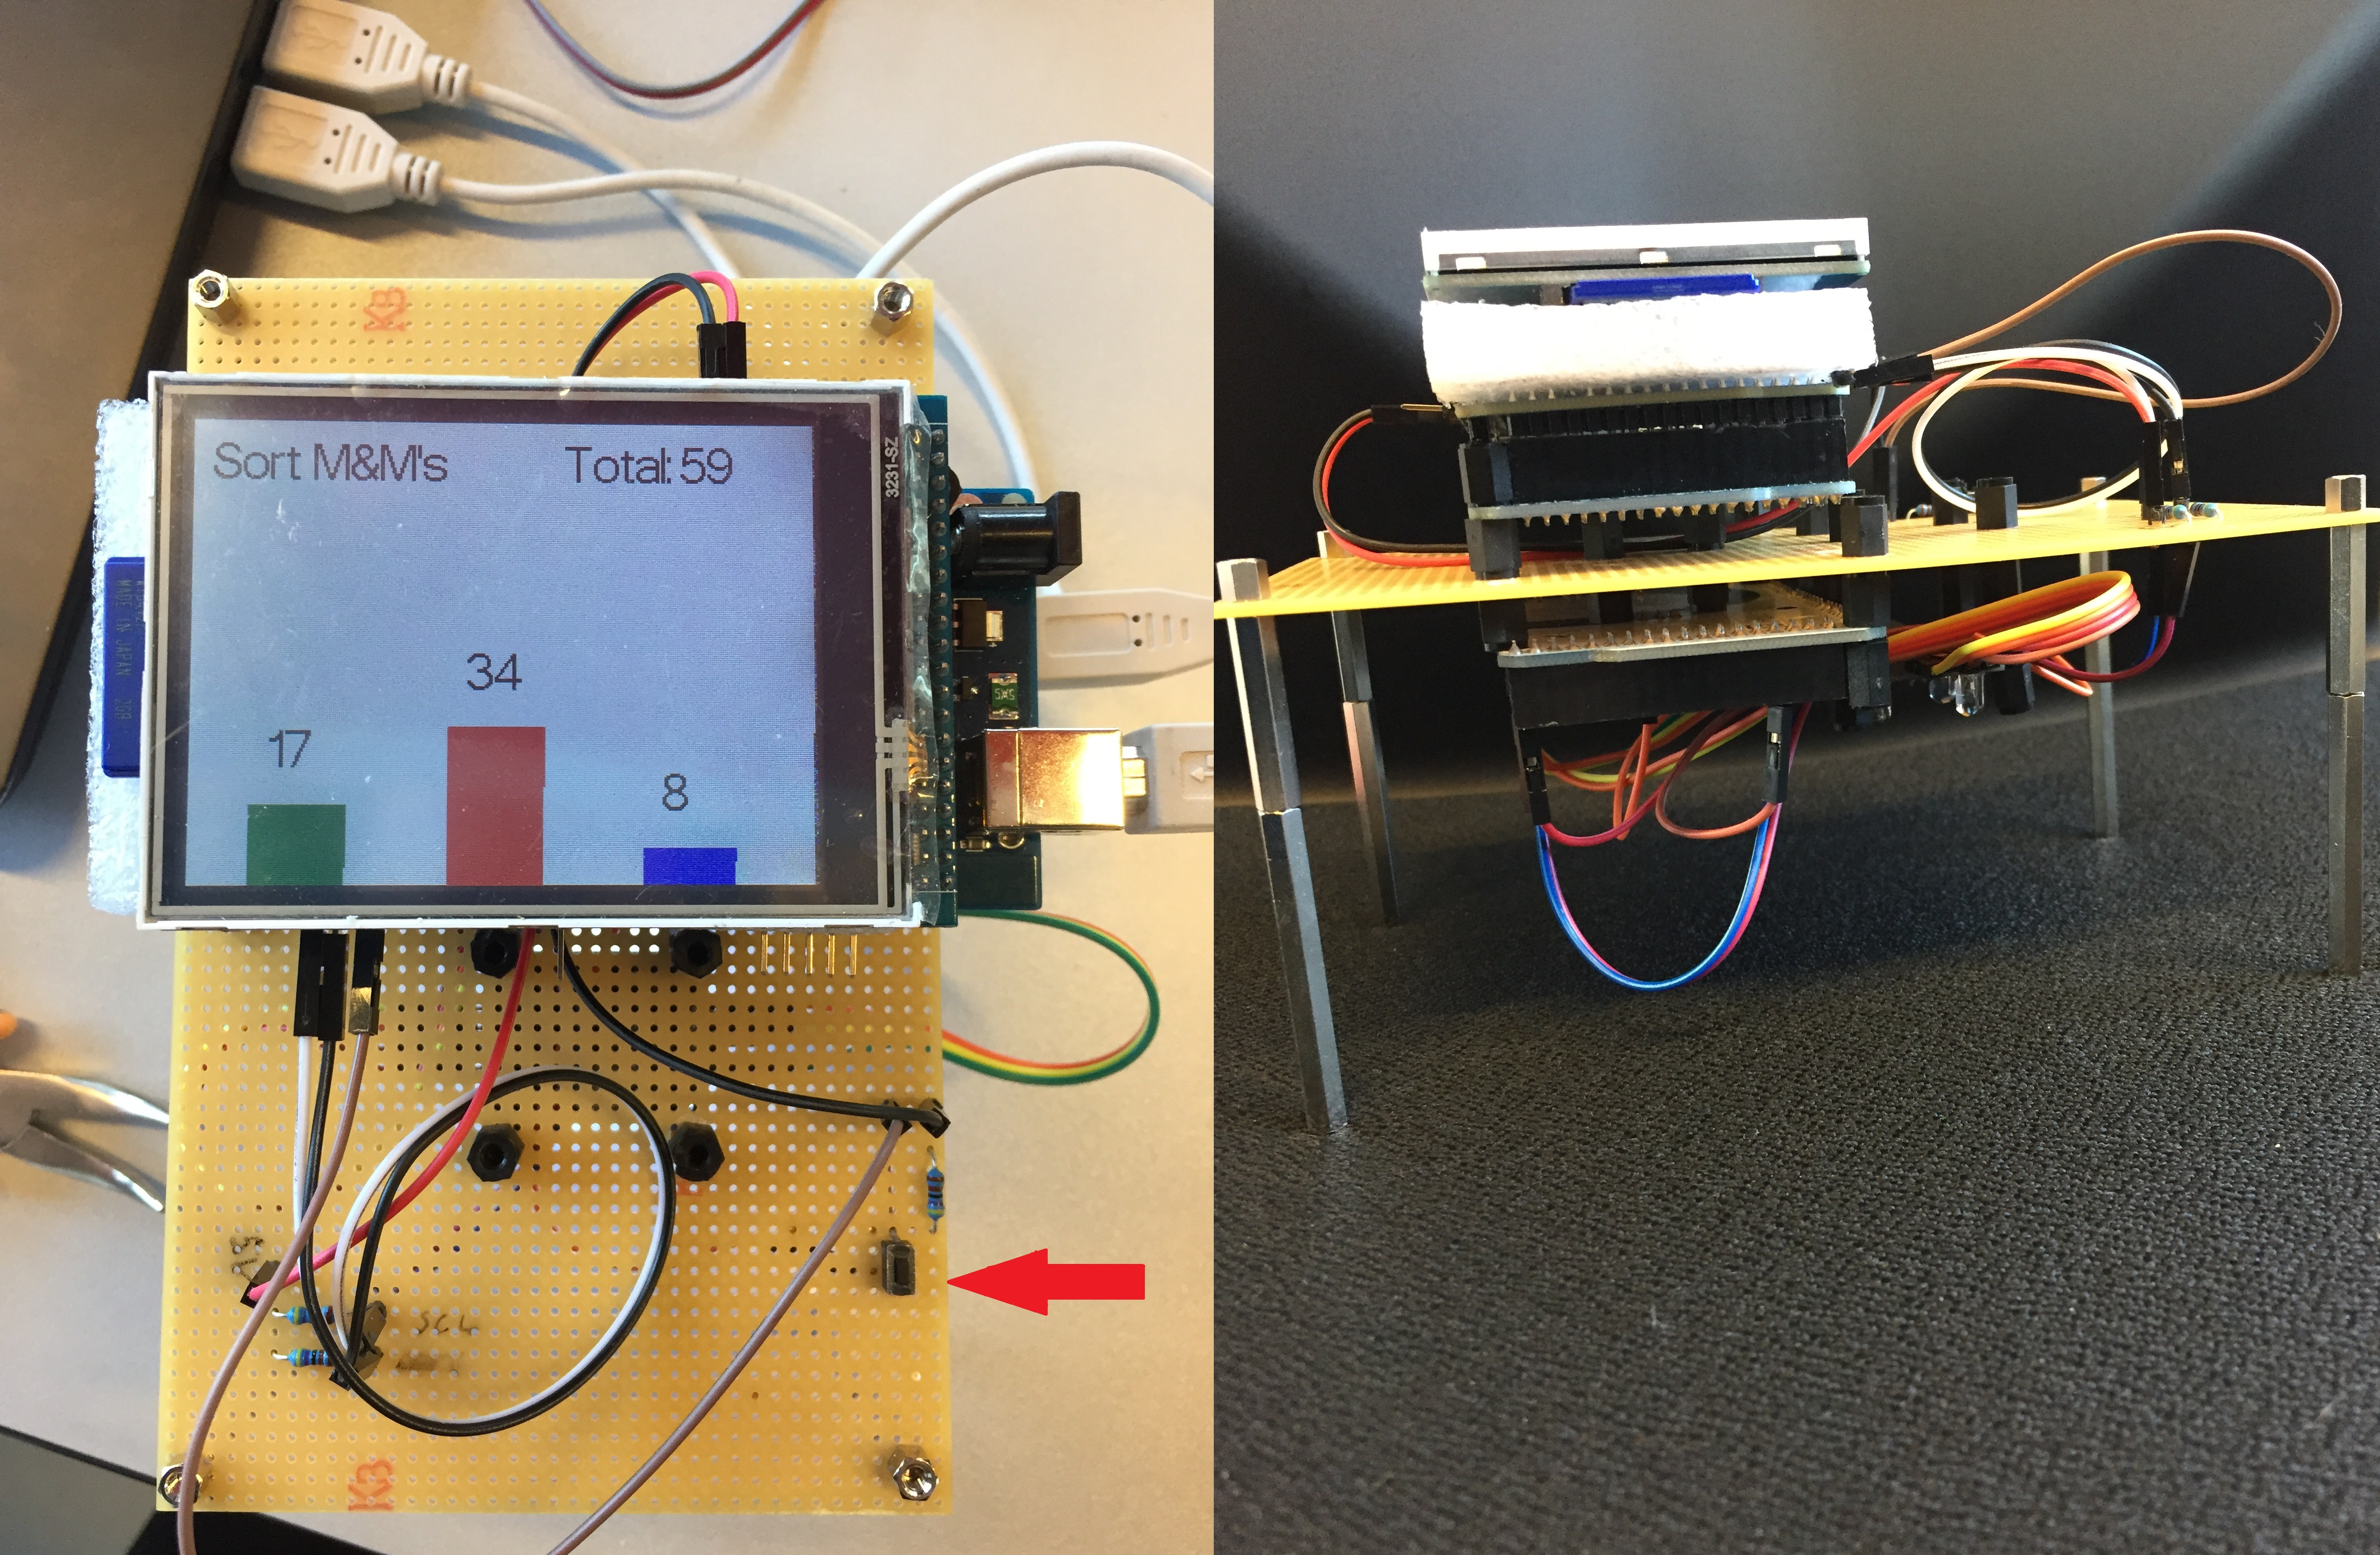
\includegraphics[width = 300pt]{Img/CSS_top_bottom.jpg}
	\caption{CSS set oppe fra og fra siden}
	\label{fig:CSS_top_bottom}
\end{figure}

Som det ses på \autoref{fig:CSS_top_bottom}, kan man se hvordan prototypen ser ud oppe fra og fra siden. Prototypen er testet ved at sætte et farvet stykke papir in under sensoren som sidder på undersiden af prototypen. Mens papiret er under sensoren, trykkes der på knappen (udfra rød pil) og den pågældende farve vil blive talt op. En film af dette kan findes blandt bilagene. Nedenunder på \autoref{fig:CSS_bottom} ses CSS nede fra. Der kan man se hvor sensoren er sat fast.


\begin{figure}[H]
	\centering
	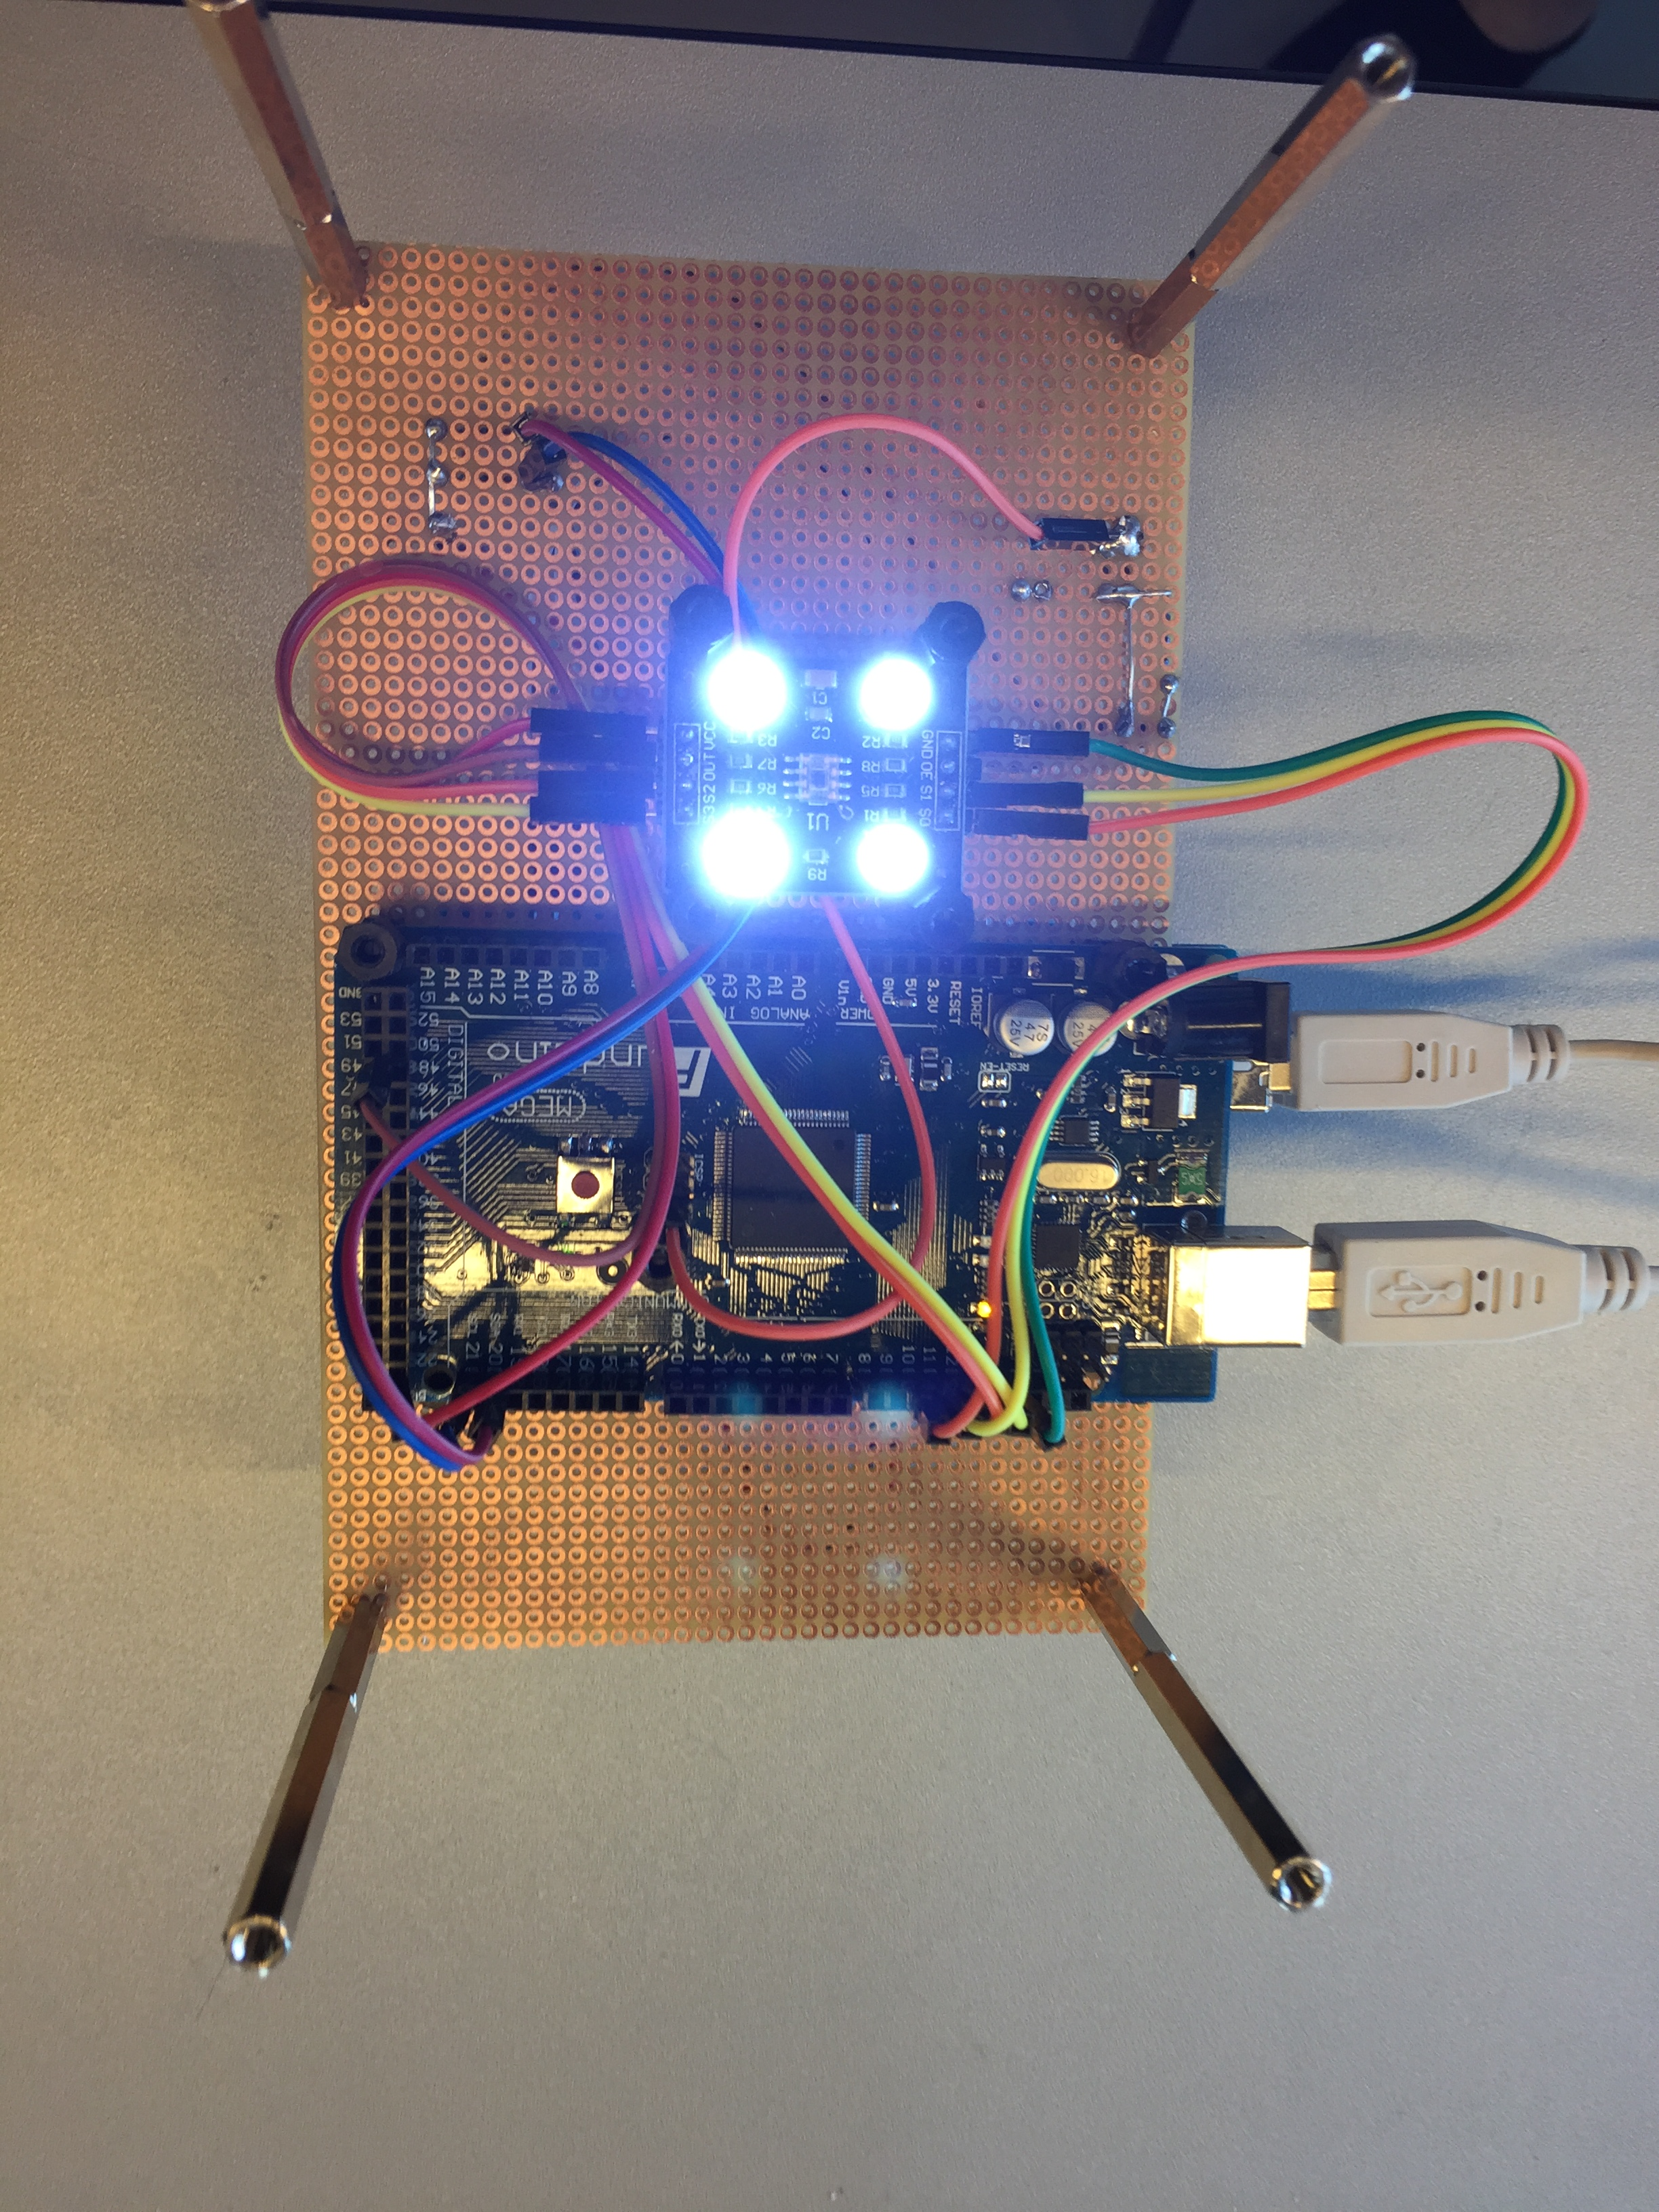
\includegraphics[width = 300pt]{Img/CSS_bottom.jpg}
	\caption{CSS nede fra}
	\label{fig:CSS_bottom}
\end{figure}
